\section{实用技巧}
本章包含许多有用的信息、实用技巧、建议和技术,这些信息在使用 SYCL 进行 C++ 编程时已被证明非常有用。 
这些主题都没有被详尽地涵盖,因此目的是提高认识并鼓励根据需要学习更多内容。

\subsection{获取代码示例和编译器}
第 1 章介绍如何获取 SYCL 编译器(例如 oneapi.com/implementations 
或 github.com/intel/llvm)以及从何处获取本书中使用的代码示例(github.com/Apress/data-parallel-CPP) 。 
再次提到这一点是为了强调尝试示例(包括进行修改!)以获得实践经验是多么有用。 
加入那些知道图 1-1 中的代码实际打印出什么内容的人吧!

\subsection{在线资源}
主要在线资源包括

\begin{itemize}
	\item sycl.tech/ 上的丰富资源

	\item 官方 SYCL 主页位于 khronos.org/sycl/,其中列出了 khronos.org/sycl/resources 上的大量资源

	\item 帮助使用 SYCL 从 CUDA 迁移到 C++ 的资源,位于tinyurl.com/cuda2sycl

	\item 迁移工具 GitHub 主页 github.com/oneapi-src/SYCLomatic
\end{itemize}

\subsection{平台模型}
支持 SYCL 的 C++ 编译器的设计方式和感觉与我们曾经使用过的任何其他 C++ 编译器一样。 
值得深入了解内部工作原理,使具有 SYCL 支持的编译器能够为主机(例如 CPU)和设备生成代码。

\begin{figure}[H]
	\centering
	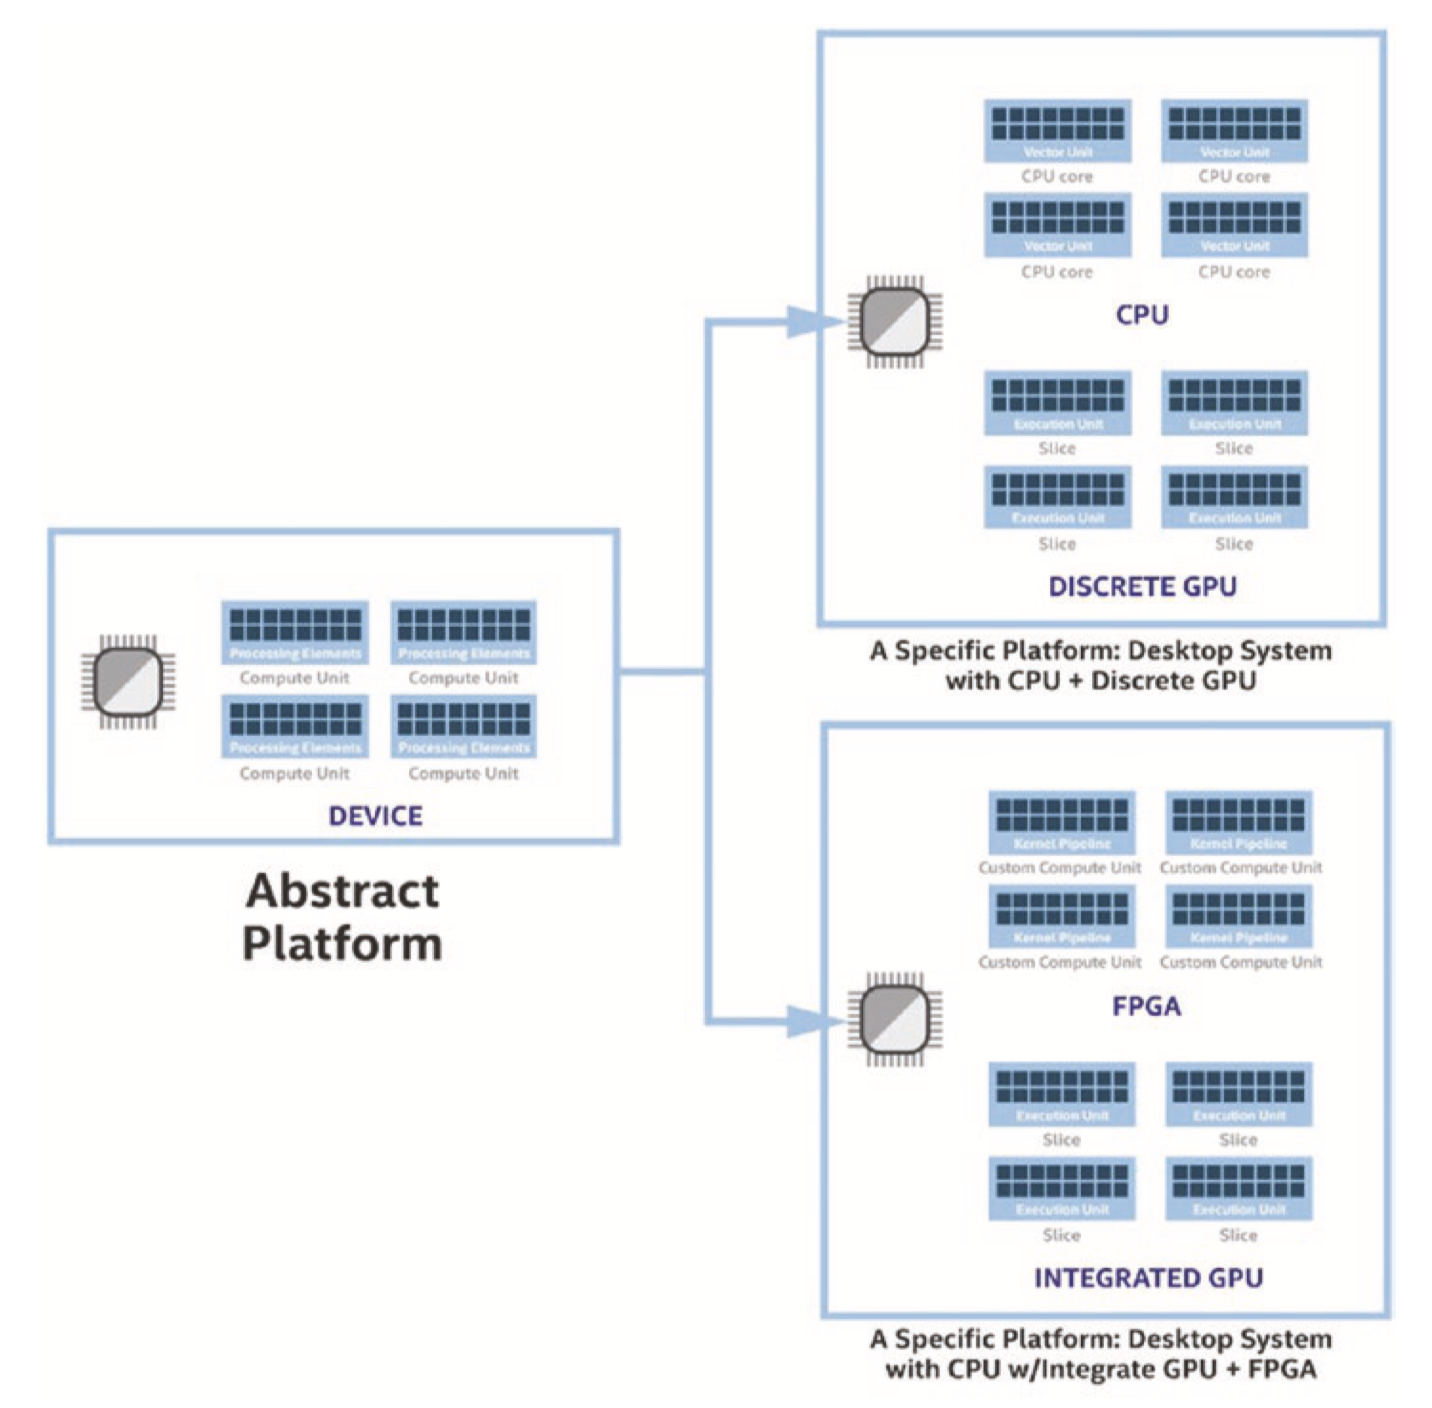
\includegraphics[width=0.9\textwidth]{figs/F13.1.png}
	\caption{\textit{平台模型:可以抽象使用,也可以具体使用 }}
\end{figure}

SYCL 使用的平台模型(图 13-1)指定了一个主机,用于协调和控制在设备上执行的计算工作。 
第 2 章介绍如何向设备分配工作,第 4 章深入介绍如何对设备进行编程。 第 12 章描述了在各个具体级别上使用平台模型。

正如我们在第 2 章中讨论的,使用正确配置的 SYCL 运行时和兼容硬件的系统中应该始终有一个设备可以运行。 
这允许在假设至少有一个设备可用的情况下编写设备代码。 
运行设备代码的设备的选择是在程序控制下的——作为程序员,
我们是否想要以及如何在特定设备上执行代码完全是我们的选择(设备选择选项将在第 12 章中讨论)。

\subsubsection{多架构二进制文件}
由于我们的目标是拥有单一源代码来支持异构机器,因此很自然地希望结果是单个可执行文件。

多架构二进制文件(又名胖二进制文件)是一个单一的二进制文件,
它已扩展为包含我们的异构机器所需的所有已编译代码和中间代码。 
多架构二进制文件的行为与我们习惯的任何其他 a.out 或 a.exe 类似,但它包含异构计算机所需的所有内容。 
这有助于自动选择为特定设备运行的正确代码的过程。 
正如我们接下来讨论的,胖二进制文件中设备代码的一种可能形式是中间格式,它将设备指令的最终创建推迟到运行时。

\subsubsection{编译模型}
SYCL 的单一源性质允许编译的行为和感觉就像常规 C++ 编译一样。 
我们不需要为设备调用额外的通道或处理捆绑设备和主机代码。 这一切都是由编译器自动为我们处理的。 
当然,出于多种原因,了解正在发生的事情的细节可能很重要。 
如果我们想要更有效地针对特定体系结构,这是有用的知识,并且了解我们是否需要调试编译过程中发生的故障也很重要。

我们将审查编译模型,以便我们在需要这些知识时接受教育。 
由于编译模型支持同时在主机和潜在多个设备上执行的代码,
因此编译器、链接器和其他支持工具发出的命令比我们习惯的 C++ 编译(仅针对一种体系结构)更复杂。 欢迎来到异构世界!

这种异构的复杂性被编译器故意隐藏起来,并且“正常工作”。

编译器可以生成类似于传统 C++ 编译器的特定于目标的可执行代码(提前(AOT)编译,有时称为离线Kernel编译),
也可以生成可以即时的中间表示( JIT)在运行时编译为特定目标。

\begin{remark}
	编译可以是“提前”(AOT)或“即时”(JIT)。
\end{remark}

只有提前知道设备目标(在我们编译程序时),编译器才能提前编译。 
使用 JIT 编译将为我们编译的程序提供更多的可移植性,但需要编译器和运行时在我们的应用程序运行时执行额外的工作。

对于大多数设备,包括 GPU,最常见的做法是依赖 JIT 编译。 
某些设备(例如 FPGA)的编译过程可能非常慢,因此实践是使用 AOT 编译。

\begin{remark}
	除非您知道使用 AOT 代码有需要(例如,FPGA)或好处,否则请使用 JIT。
\end{remark}

默认情况下,当我们为大多数设备编译代码时,设备代码的输出以中间形式存储。 
在运行时,系统上的设备驱动程序将及时将中间形式编译为代码以在设备上运行,以匹配系统上可用的内容。

\begin{remark}
	与 AOT 代码不同,JIT 代码的目标是能够在运行时进行编译,以使用系统上的任何设备。
	这可能包括最初将程序编译为 JIT 代码时不存在的设备。
\end{remark}

我们可以要求编译器针对特定设备或设备类别提前进行编译。 
这样做的优点是节省运行时间,但缺点是增加了编译时间和使二进制文件变得更胖! 提前编译的代码不如即时编译的代码那么可移植,
因为它无法在运行时进行调整以匹配可用的硬件。 我们可以将两者都包含在我们的二进制文件中,以获得 AOT 和 JIT 的好处。

\begin{remark}
	为了最大限度地提高可移植性,即使包含一些 AOT 代码,我们也喜欢在我们的二进制文件中加入 JIT 代码。
\end{remark}

提前针对特定设备进行编译还可以帮助我们在构建时检查我们的程序是否应该在该设备上运行。 
使用即时编译,程序可能会在运行时编译失败(可以使用第 5 章中的机制捕获)。 
在本章即将到来的“调试”部分中有一些调试技巧,第 5 章详细介绍了如何在运行时捕获这些错误,以避免要求我们的应用程序中止。

\begin{figure}[H]
	\centering
	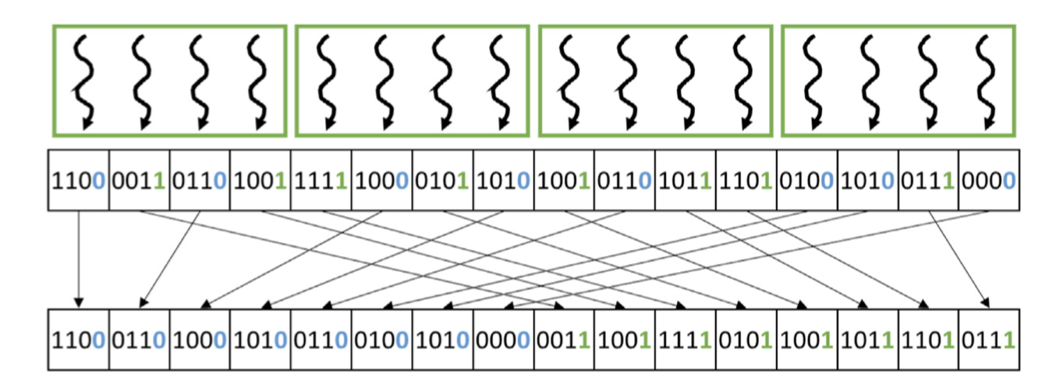
\includegraphics[width=0.9\textwidth]{figs/F13.2.png}
	\caption{\textit{编译过程:JIT和AOT选项 }}
\end{figure}

图 13-2 说明了从源代码到 fat 二进制文件(可执行文件)的编译过程。 
无论我们选择什么组合,都会组合成一个胖二进制文件。 
当应用程序执行时,运行时会使用 fat 二进制文件(它是我们在主机上执行的二进制文件!)。 
有时,我们可能希望在单独的编译中为特定设备编译设备代码。 
我们希望这样一个单独编译的结果最终能够合并到我们的胖二进制文件中。 
当完整编译(进行完整综合布局布线)时间可能非常长时,这对于 FPGA 开发非常有用,
而且实际上这是 FPGA 开发的一项要求,以避免需要在运行时系统上安装综合工具。 
图 13-3 显示了支持此类需求的捆绑/分拆活动的流程。 
我们总是可以选择一次编译所有内容,但在开发过程中,中断编译的选项可能非常有用。

\begin{figure}[H]
	\centering
	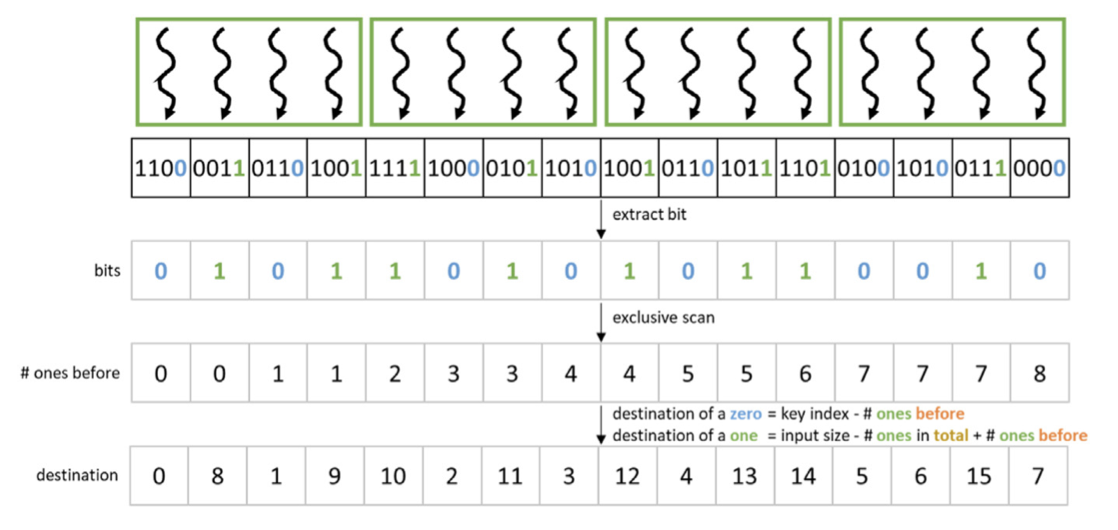
\includegraphics[width=0.9\textwidth]{figs/F13.3.png}
	\caption{\textit{编译过程:卸载 bundler/unbundler }}
\end{figure}

每个支持 SYCL 的 C++ 编译器都有一个具有相同目标的编译模型,但具体的实现细节会有所不同。 
此处显示的具体图表由 DPC++ 编译器工具链实现者提供。

\subsection{上下文:需要了解的重要事项}
正如第 6 章中提到的,上下文代表我们可以在其上执行Kernel的一个设备或一组设备。 
我们可以将上下文视为运行时存储有关其正在执行的操作的某些状态的方便位置。 
除了在大多数 SYCL 程序中传递上下文之外,程序员不太可能直接与上下文交互。

设备可以细分为子设备。 这对于划分问题很有用。 
由于子设备被完全视为设备(相同的 C++ 类型),因此我们所说的有关分组设备的所有内容也适用于子设备。

SYCL 抽象地认为设备在平台中分组在一起。 在平台内,设备可以通过共享内存等方式进行交互。 
属于同一上下文的设备必须能够使用某种机制访问彼此的全局内存。 
仅当设备处于同一上下文中时,才能在设备之间共享 SYCL USM 内存(第 6 章)。 
USM 内存分配绑定到上下文,而不是设备,因此一个上下文中的 USM 分配无法被其他上下文访问。 
因此,USM 分配仅限于在单个上下文(可能是设备的子集)内使用。

上下文并不抽象硬件不能支持的内容。 
例如,我们无法创建一个上下文来包含两个不能彼此共享内存的 GPU。 
并非所有从同一平台公开的设备都需要能够在同一上下文中分组在一起。

当我们创建队列时,我们可以指定我们希望将其放置在哪个上下文中。 
默认情况下,DPC++ 编译器项目为每个平台实现默认上下文,并自动将新队列分配给默认上下文。 
其他 SYCL 编译器可以自由地执行相同的操作,但标准并不要求这样做。

\begin{remark}
	上下文的创建成本很高,而创建上下文的成本越低,我们的应用程序就越高效。
\end{remark}

将给定平台的所有设备始终放置在同一上下文中具有两个优点:
(1)由于创建上下文的成本很高,因此我们的应用程序更加高效; (2) 允许硬件支持的最大共享(例如USM)。

\subsection{将 SYCL 添加到现有 C++ 程序}
将并行性的适当利用添加到现有 C++ 程序中是使用 SYCL 的第一步。 
如果 C++ 应用程序已经在利用并行执行,这可能是一个好处,也可能是一个令人头疼的问题。 
这是因为我们将应用程序的工作划分为并行执行的方式极大地影响了我们可以用它做什么。 
当程序员谈论重构程序并行性时,他们指的是重新安排程序内的执行流和数据流,以使其准备好利用并行性。 
这是一个复杂的话题,我们只会简单地讨论一下。 
关于如何准备并行性应用程序,没有一刀切的答案,但有一些值得注意的技巧。

当向 C++ 应用程序添加并行性时,考虑的一个简单方法是在程序中找到并行机会最大的孤立点。 
我们可以从那里开始修改,然后根据需要继续在其他区域添加并行性。 
一个复杂的因素是重构(即重新安排程序流程和重新设计数据结构)可能会提高并行性的机会。

一旦我们在程序中找到并行机会最大的孤立点,
我们就需要考虑如何在程序中的该点使用 SYCL。 这就是本书其余部分所教导的。

从高层次来看,引入并行性的关键步骤包括以下内容:

\begin{enumerate}
	\item 并发安全(在传统CPU编程中通常称为线程安全):
	调整所有共享可变数据(可以更改并可能同时执行操作的数据)的使用,以防止数据竞争。 参见第 19 章。

	\item 引入并发和/或并行性。

	\item 并行性调整(最佳扩展、吞吐量或延迟优化)。
\end{enumerate}

首先考虑步骤\#1 很重要。 许多应用程序已经针对并发性进行了重构,但许多应用程序还没有。 
将 SYCL 作为并行性的唯一来源,我们重点关注Kernel中使用的数据以及可能与主机共享的数据的安全性。 
如果我们的程序中有其他引入并行性的技术(OpenMP、MPI、TBB 等),那么这就是我们 SYCL 编程之外的另一个问题。 
值得注意的是,可以在单个程序中使用多种技术。
SYCL 不需要是程序中并行性的唯一来源。 本书不涉及与其他并行技术混合的高级主题。

\subsection{使用多个编译器时的注意事项}
支持 SYCL 的 C++ 编译器还支持与其他 C++ 编译器的目标代码(库、目标文件等)链接。 
一般来说,使用多个编译器出现的任何问题都与任何 C++ 编译器相同,需要考虑名称修改、针对相同的标准库、对齐调用约定等。
这些是我们在混合和使用时必须处理的相同问题。 匹配其他语言(例如 Fortran 或 C)的编译器。

此外,应用程序必须使用用于构建程序的编译器附带的 SYCL 运行时。 
混合和匹配 SYCL 编译器和 SYCL 运行时并不安全 - 不同的运行时对于重要的 SYCL 对象可能有不同的实现和数据布局。

\begin{remark}
	SYCL 与非 SYCL 源语言的互操作性是指 SYCL 能够使用用其他编程语言(如 OpenCl、C 或 CUDA)编写的Kernel函数
	或设备函数,或者使用由其他编译器预编译的中间表示形式的代码。
	有关与非 SYCL 源语言的互操作性的更多信息,请参阅第 20 章。
\end{remark}

最后,还需要使用用于编译 SYCL 设备代码的相同编译器工具链来完成编译的链接阶段。 
使用来自不同编译器工具链的链接器进行链接不会产生功能性程序,
因为不支持 SYCL 的编译器将不知道如何正确集成主机和设备代码。

\subsection{调试}
本节传达了一些适度的调试建议,以缓解调试并行程序所特有的挑战,尤其是针对异构机器的并行程序。

我们永远不应该忘记,当应用程序在 CPU 设备上运行时,我们可以选择对其进行调试。 
该调试技巧在第 2 章中被描述为方法\#2。
由于设备的体系结构通常比通用 CPU 包含更少的调试挂钩,因此工具通常可以更精确地探测 CPU 上的代码。 
在 CPU 上运行所有内容时的一个重要区别是,许多与同步相关的错误将会消失,包括在主机和设备之间来回移动内存。 
虽然我们最终需要调试所有此类错误,但这可以允许增量调试,因此我们可以在其他错误之前解决一些错误。 
经验表明,尽可能频繁地在我们的目标设备上运行非常重要,
就像在调试过程中利用 CPU(和其他设备)的可移植性一样,运行多个设备将有助于暴露问题,并有助于隔离是否存在问题。 
我们遇到的错误是特定于设备的。

\begin{remark}[调试提示]
在 CPU 上运行是一个功能强大的调试工具。
\end{remark}

在主机上运行所有代码时,工具通常更容易检测和消除并行编程错误,特别是数据争用和死锁。 
令我们懊恼的是,当在主机和设备的组合上运行时,我们经常会看到由于此类并行编程错误而导致的程序失败。 
当出现此类问题时,记住退回到仅 CPU 是一个强大的调试工具,这一点非常有用。 
值得庆幸的是,SYCL 经过精心设计,让我们可以轻松访问此选项。

\begin{remark}[调试提示]
如果程序处于死锁状态,请检查主机访问器是否被正确销毁,以及Kernel中的工作项是否遵循 SYCL 规范中的同步规则。
\end{remark}

当我们开始调试时,以下编译器选项是一个好主意:

\begin{itemize}
	\item -g:将调试信息放入输出中

	\item -ferror-limit=1:在将 C++ 与模板库(例如 SYCL 大量使用的模板库)一起使用时保持理智

	\item -Werror -Wall -Wpedantic:让编译器强制执行良好的编码,以帮助避免生成错误的代码以在运行时进行调试
\end{itemize}

我们确实不需要仅仅为了将 C++ 与 SYCL 一起使用而陷入修复迂腐警告的困境,因此选择不使用 -Wpedantic 是可以理解的。

当我们让代码在运行时即时编译时,我们可以检查一些代码。 
这高度依赖于我们的编译器使用的层,因此查看编译器文档以获取建议是一个好主意。

\subsubsection{调试死锁和其他同步问题}
并行编程依赖于并行发生的工作之间的适当协调。 
数据使用需要在数据准备好使用时进行控制——这种数据依赖关系需要在我们的程序逻辑中进行编码以获得正确的行为。

当我们的同步/依赖逻辑发生错误时,调试依赖问题(尤其是 USM)可能是一个挑战。 
我们可能会看到程序挂起(永远不会完成)或间歇性地生成错误信息。 
在这种情况下,我们可能会看到诸如“它会失败,直到我在调试器中运行它,然后它才能完美运行!”之类的行为。 
这种间歇性故障通常源于未通过等待、锁定、队列提交之间的显式依赖关系等方式正确同步的依赖关系。

有用的调试技术包括

\begin{itemize}
	\item 从无序队列切换到有序队列

	\item 散布queue.wait()调用
\end{itemize}

在调试时使用其中一个或两个可以帮助识别依赖信息可能丢失的位置。 
如果此类更改使程序故障发生变化或消失,则强烈暗示我们的同步/依赖逻辑中有问题需要纠正。 
修复后,我们将删除这些临时调试措施。

\subsubsection{调试Kernel代码}
调试Kernel代码时,首先在 CPU 设备上运行(如第 2 章所述)。 
第 2 章中的设备选择器代码可以轻松修改为接受运行时选项或编译时选项,以便在调试时将工作重定向到主机设备。

\begin{figure}[H]
	\centering
	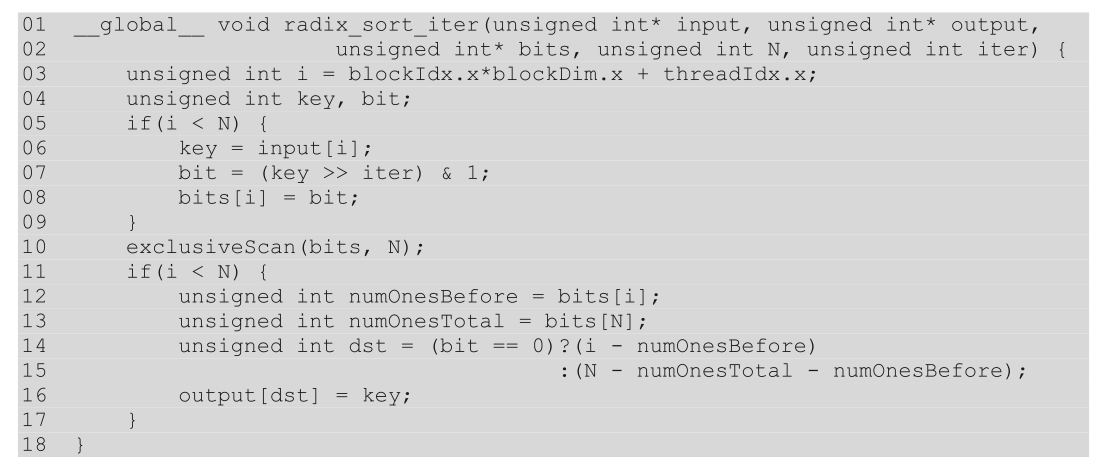
\includegraphics[width=0.9\textwidth]{figs/F13.4.png}
	\caption{\textit{sycl::stream }}
\end{figure}

当调试Kernel代码时,SYCL 定义了一个可以在Kernel中使用的 C++ 风格的流(图 13-4)。 
DPC++ 编译器还提供了 C 风格 printf 的实验性实现,它具有有用的功能,但有一些限制。

在调试Kernel代码时,经验鼓励我们将断点放在parallel\_for之前或parallel\_for内部,
但实际上不要放在parallel\_for上。 即使在执行下一个操作之后,放置在parallel\_for 上的断点也可以多次触发断点。 
此 C++ 调试建议适用于许多模板扩展,例如 SYCL 中的模板扩展,
其中模板调用上的断点在编译器扩展时将转换为一组复杂的断点。 
实现可能有一些方法可以缓解这个问题,但这里的关键点是,
我们可以通过不在parallel\_for本身上精确设置断点来避免所有实现上的一些混乱。

\subsubsection{调试运行时故障}
当即时编译时发生运行时错误时,我们要么正在处理明确使用可用硬件无法支持的功能(例如,fp16 或 simd8)的情况,
要么是编译器/运行时错误,要么是我们意外地使用了可用硬件无法支持的功能(例如,fp16 或 simd8)。 
编写的无意义内容直到运行时出错并创建难以理解的运行时错误消息后才被检测到。 
在这三种情况下,深入研究这些错误可能有点令人生畏。 
值得庆幸的是,即使是粗略的观察也可以让我们更好地了解导致特定问题的原因。 
它可能会产生一些额外的知识来指导我们避免该问题,或者它可能只是帮助我们向编译器团队提交一份简短的错误报告。 
无论哪种方式,了解一些可以提供帮助的工具都很重要。

我们的程序的指示运行时失败的输出可能类似于以下示例:

terminate called after throwing an instance of 'sycl::\_V1::runtime\_error' what(): Native API failed. Native API returns: ...

or

terminate called after throwing an instance of 'sycl::\_V1::compile\_program\_error' what(): The program was built for 1 devices 

...

error: Kernel compiled with required subgroup size 8, which is unsupported on this platform in kernel: 'typeinfo name for main::'lambda'(sycl::\_V1::nd\_item<2>)' error: backend compiler failed build.

-11 (PI\_ERROR\_BUILD\_PROGRAM\_FAILURE)

在这里看到此类异常让我们知道我们的主机程序可以被构造为捕获此错误。 
第一个显示了访问本机不支持的任何 API 时出现的一些包罗万象的错误(在这种情况下,它使用了平台不支持的主机端内存分配); 
第二个更容易认识到 SIMD8 是为不支持它的设备指定的(在本例中它支持 SIMD16)。 
运行时编译器失败不需要中止我们的应用程序; 我们可以抓住它们,或者编写代码来避免它们,或者两者兼而有之。 
第 5 章深入探讨这个主题。

当我们看到运行时故障并且在快速调试时遇到困难时,值得尝试使用提前编译进行重建。 
如果我们的目标设备具有提前编译选项,那么这可能是一件容易尝试的事情,可能会产生更容易理解的诊断。 
如果我们的错误可以在编译时而不是 JIT 或运行时看到,那么通常会在编译器的错误消息中找到更有用的信息,
而不是我们通常从 JIT 或运行时看到的少量错误信息。

\begin{figure}[H]
	\centering
	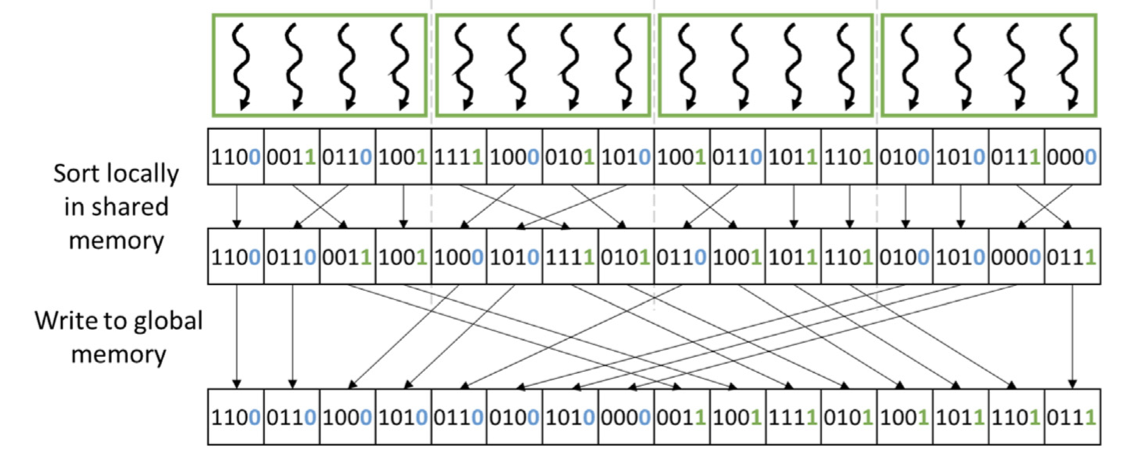
\includegraphics[width=0.9\textwidth]{figs/F13.5.png}
	\caption{\textit{DPC++高级调试选项 }}
\end{figure}

图 13-5 列出了编译器或运行时支持的两个标志和附加环境变量(在 Windows 和 Linux 上受支持),以帮助进行高级调试。 
这些是 DPC++ 编译器特定的高级调试选项,用于检查和控制编译模型。 
本书中没有讨论或使用它们; 
GitHub 项目在 intel.github.io/llvm-docs/EnvironmentVariables.html 
和tinyurl.com/IGCoptions 上对它们进行了在线详细解释。

本书中没有对这些选项进行更多描述,但这里提到它们是为了根据需要开辟这种高级调试的途径。 
这些选项可以让我们深入了解如何解决问题或错误。 我们的源代码有可能无意中触发了一个问题,可以通过更正源代码来解决。 
否则,使用这些选项是为了对编译器本身进行非常高级的调试。 
因此,它们与编译器开发人员的关系比与编译器用户的关系更多。 
一些高级用户发现这些选项很有用; 因此,它们在这里被提及,并且在本书中不再被提及。 
要深入了解,请参阅 DPC++ 编译器 GitHub 项目 intel.github.io/llvm-docs/EnvironmentVariables.html。

\begin{remark}[调试提示]
当其他选项用尽并且我们需要调试运行时问题时,我们会寻找可能为我们提供原因提示的转储工具。
\end{remark}

\subsubsection{队列分析和由此产生的计时功能}
许多设备支持队列分析(device::has(aspect::queue\_profiling)——有关一般方面的更多信息,请参阅第 12 章。
一个简单而强大的接口可以轻松访问有关队列提交、实际执行开始的详细计时信息 设备上的完成、设备上的完成以及命令的完成。
与使用主机计时机制(例如 chrono)相比,此分析对于设备计时更加精确,因为它们通常不包括主机到设备的数据传输时间。 
请参阅图 13-6 和图 13-7 中所示的示例,以及图 13-8 中所示的示例输出。
图 13-8 中所示的示例输出说明了此技术的可能性,但尚未优化,不应使用 以任何方式代表任何特定系统选择的优点。

aspect::queue\_profiling 方面指示设备通过 property::queue::enable\_profiling 支持队列分析。

对于此类设备,我们可以在构造队列时指定 property::queue::enable\_profiling — 
属性列表是队列构造函数的可选最终参数。 这样做会激活 SYCL 运行时捕获提交到该队列的命令组的分析信息。 
然后通过 SYCL 事件类 get\_profiling\_info 成员函数提供捕获的信息。 
如果队列的关联设备没有aspect::queue\_profiling,
这将导致构造函数抛出带有errc::feature\_not\_supported错误代码的同步异常。

可以使用事件类的 get\_profiling\_info 成员函数来查询事件的分析信息,
并指定 info::event\_profiling 中枚举的分析信息参数之一。 
每个信息参数的可能值和任何限制在与事件关联的 SYCL 后端的规范中定义。 
info::event\_profiling 中的所有信息参数均在 SYCL 规范标题为“SYCL 事件类的分析信息描述符”的表中指定,
并且 info::event\_profiling 的概要在规范附录“事件信息描述符”下描述。

每个分析描述符返回一个时间戳,表示自某些实现定义的时间基准以来已经过去的纳秒数。 
共享同一后端的所有事件都保证共享相同的时基; 
因此,来自同一后端的两个时间戳之间的差异产生了这些事件之间经过的纳秒数。

最后一点,我们提醒您,启用事件分析确实会增加开销,
因此最佳实践是在开发或调整期间启用它,然后在生产中禁用它。

\begin{remark}
	由于开销很小,请仅在开发或优化期间启用队列分析,而对生产环境禁用。
\end{remark}

\begin{figure}[H]
	\centering
	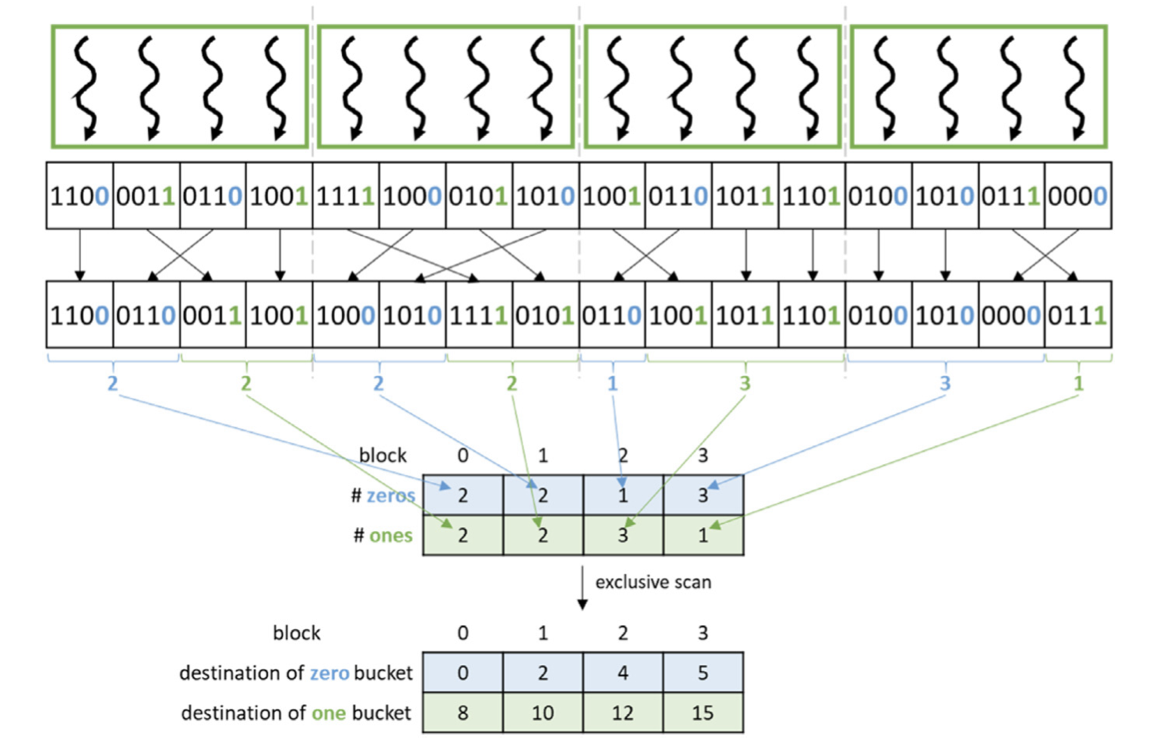
\includegraphics[width=0.9\textwidth]{figs/F13.6.png}
	\caption{\textit{设置为使用队列分析 }}
\end{figure}

\begin{figure}[H]
	\centering
	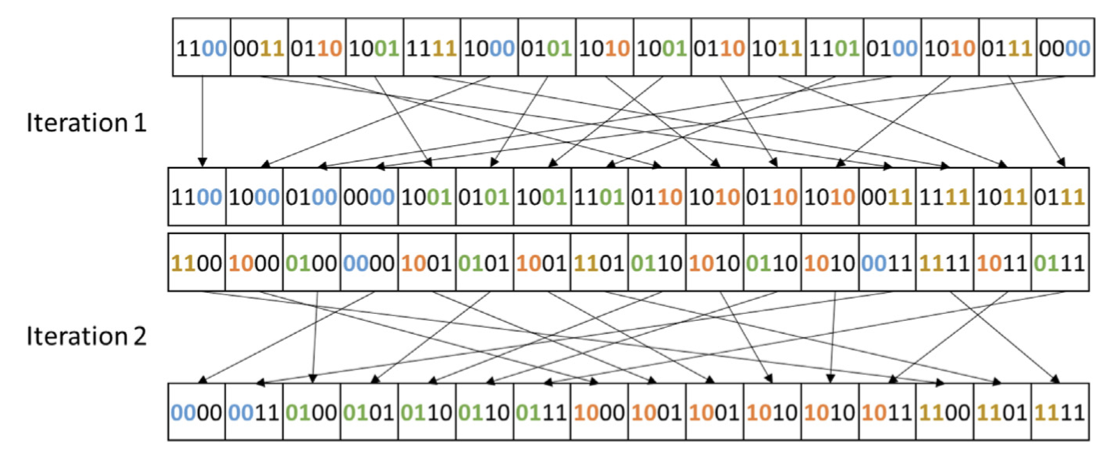
\includegraphics[width=0.9\textwidth]{figs/F13.7.png}
	\caption{\textit{使用队列分析 }}
\end{figure}

\begin{figure}[H]
	\centering
	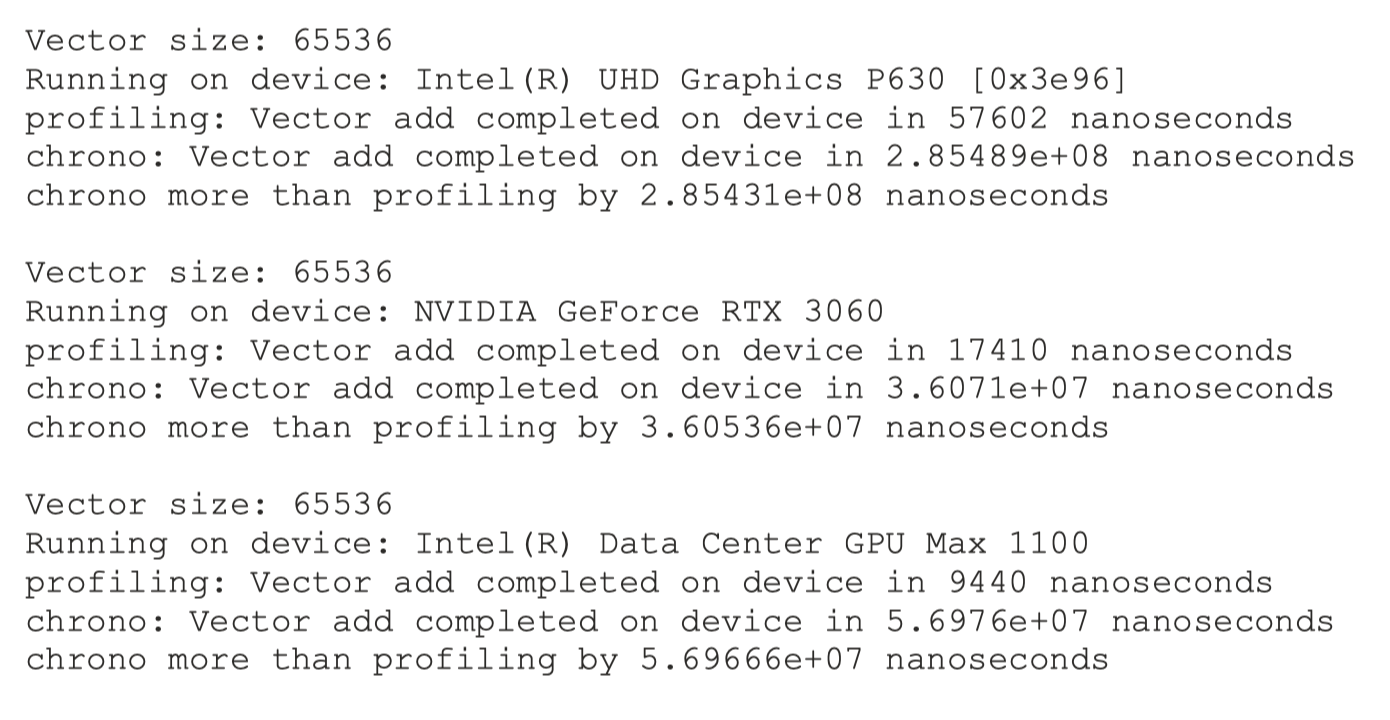
\includegraphics[width=0.9\textwidth]{figs/F13.8.png}
	\caption{\textit{队列分析示例的三个示例输出 }}
\end{figure}

\subsubsection{跟踪和分析工具接口}
跟踪和分析工具可以帮助我们了解应用程序中的运行时行为,并且通常可以揭示改进算法的机会。 
见解通常是可移植的,因为它们可以推广到各种设备,
因此我们建议在您喜欢的任何平台上使用您认为最有价值的任何跟踪和分析工具。 
当然,微调任何平台可能需要在相关平台上进行。 
对于最大程度的便携应用,我们鼓励首先寻找机会进行调整,并着眼于使任何调整尽可能便携。

当我们的 SYCL 程序在 OpenCL 运行时之上运行并使用 OpenCL 后端时,
我们可以使用 OpenCL 拦截层运行我们的程序:github.com/intel/opencl-intercept-layer。 
这是一个可以检查、记录和修改应用程序(或更高级运行时)生成的 OpenCL 命令的工具。 
它支持很多控件,但最初设置的好控件是 ErrorLogging、BuildLogging,
也许还有 CallLogging(尽管它会生成大量输出)。 使用 DumpProgramSPIRV 可以进行有用的转储。 
OpenCL 拦截层是一个单独的实用程序,不属于任何特定 OpenCL 实现的一部分,因此它可以与许多 SYCL 编译器配合使用。

还有许多其他优秀工具可用于收集 SYCL 开发人员常用的性能数据。 
它们是开源的 (github.com/intel/pti-gpu) 以及帮助我们入门的示例。

两个最流行的工具如下:

\begin{itemize}
	\item onetrace:用于 OpenCL 和零级后端的主机和设备跟踪工具,
	支持 DPC++(适用于 CPU 和 GPU)和 OpenMP GPU 卸载

	\item oneprof:适用于 OpenCL 和零级后端的 GPU 硬件指标收集工具,支持 DPC++ 和 OpenMP* GPU 卸载
\end{itemize}

这两种工具都使用来自检测运行时的信息,因此它们适用于 GPU 和 CPU。 
使用这些运行时的编译器中的 SYCL、ISPC 和 OpenMP 支持都可以从这些工具中受益。 
请查阅网站上的工具,了解它们对您的使用的适用性。 
一般来说,我们可以找到一个受支持的平台,并使用这些工具来了解有关您的程序的有用信息,即使我们目标的每个平台都不支持。 
我们学到的关于程序的大部分知识在任何地方都是有用的。

\subsection{初始化数据并访问Kernel输出}
在本节中,我们将深入探讨一个导致 SYCL 新用户感到困惑的主题,
该主题会导致我们作为新 SYCL 开发人员遇到的最常见(根据我们的经验)的第一个错误。

简而言之,当我们从主机内存分配(例如数组或向量)创建Buffer时,在Buffer被销毁之前我们无法直接访问主机分配。 
在Buffer的整个生命周期内,Buffer拥有在构造时传递给它的任何主机分配。 
很少使用允许我们在Buffer仍处于活动状态时访问主机分配的机制(例如Buffer互斥体),
但这些高级功能无助于解决此处描述的早期错误。

\begin{remark}[每个人都会犯这个错误——知道这一点可以帮助我们快速调试它,而不是长时间纠结它!!]
如果我们从主机内存分配构造Buffer,则在Buffer被销毁之前,我们不能直接访问主机分配!
当它处于活动状态时,Buffer拥有分配。了解Buffer范围和范围内的规则!
\end{remark}

当主机程序访问主机分配而Buffer仍然拥有该分配时,会出现一个常见错误。 
一旦发生这种情况,所有的赌注都会消失,因为我们不知道Buffer使用分配的目的是什么。 
如果数据不正确,请不要感到惊讶 - 我们尝试从中读取输出的Kernel可能还没有开始运行! 
如第 3 章和第 8 章所述,SYCL 是围绕异步任务图机制构建的。 
在尝试使用任务图操作的输出数据之前,我们需要确保已达到代码中执行图的同步点并使数据可供主机使用。 
Buffer破坏和主机访问器的创建都是导致此同步的操作。

\begin{figure}[H]
	\centering
	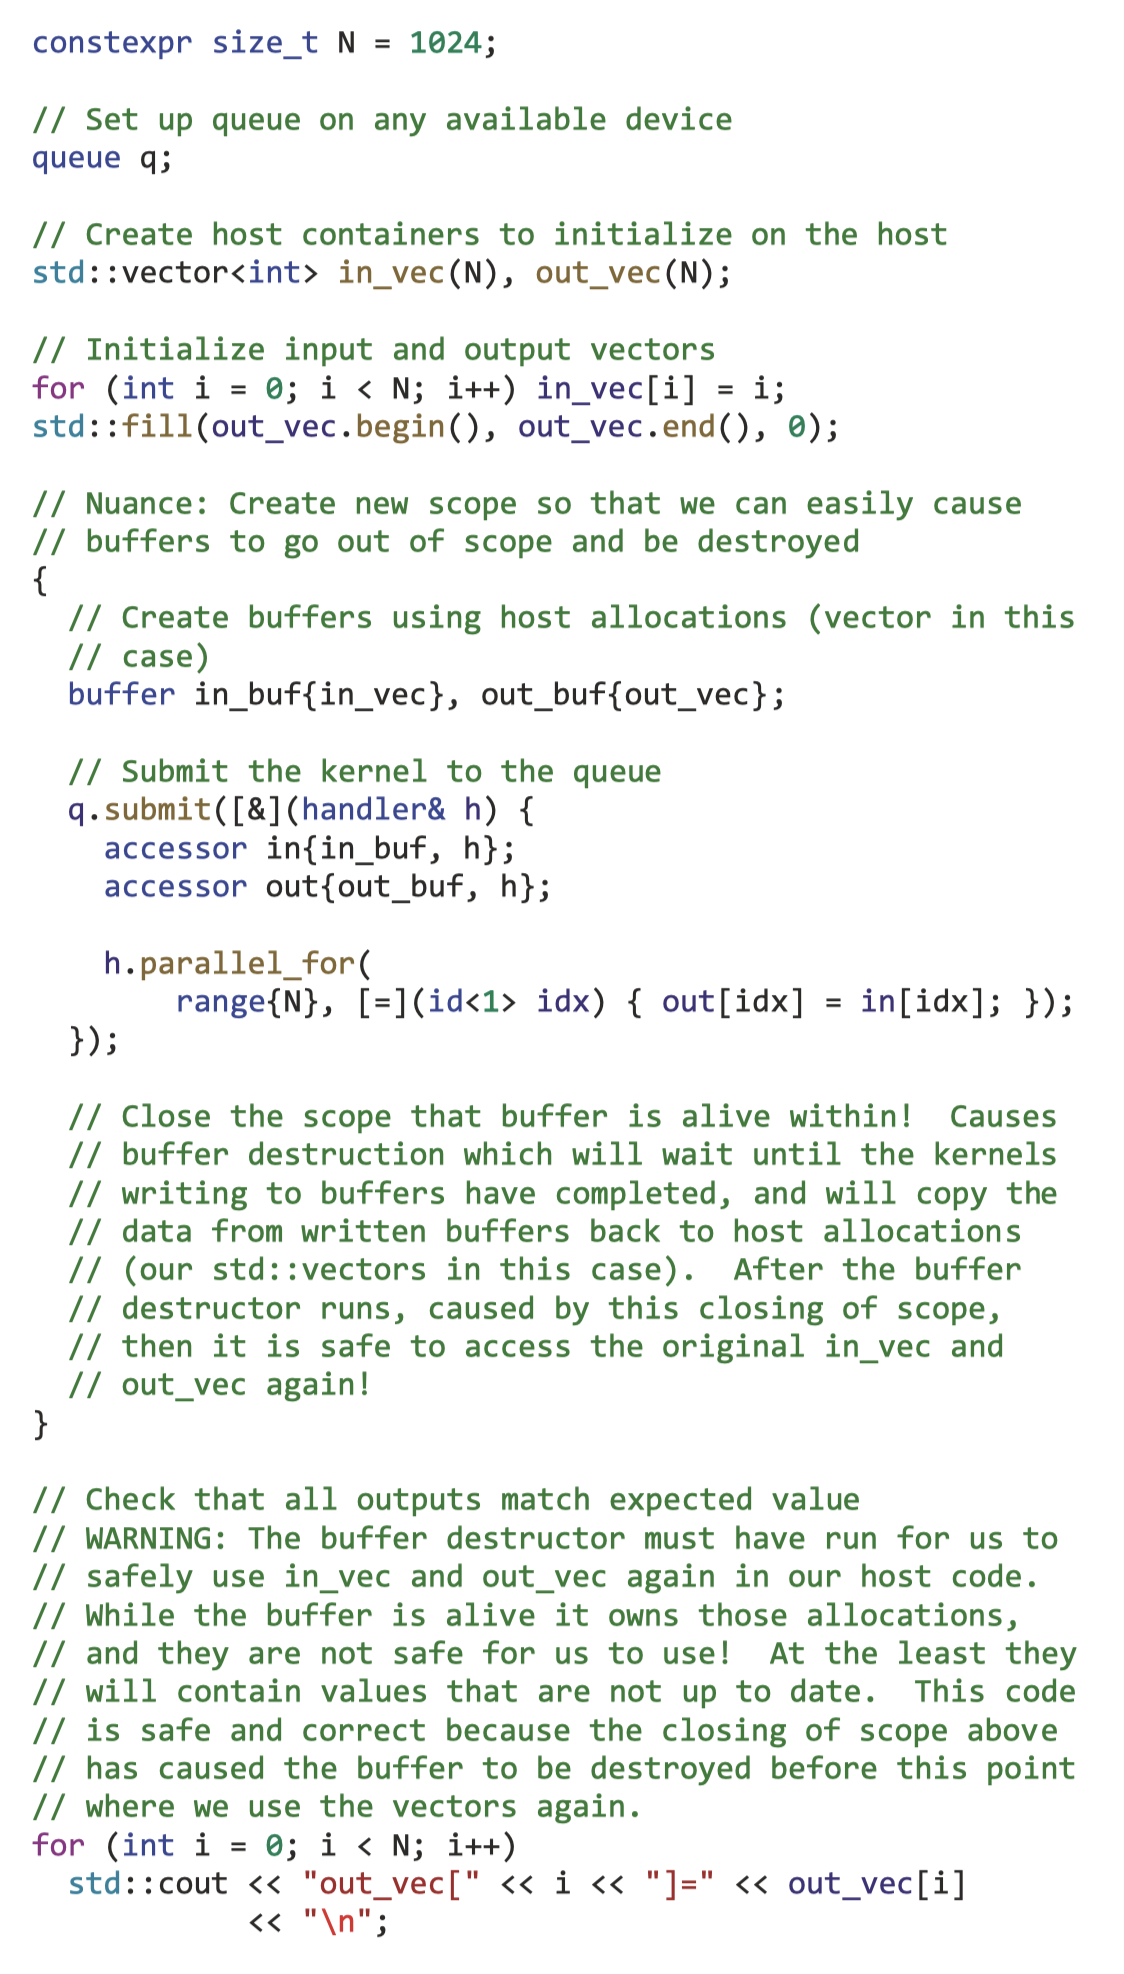
\includegraphics[width=0.9\textwidth]{figs/F13.9.png}
	\caption{\textit{常见模式:从主机分配创建Buffer }}
\end{figure}

图 13-9 显示了我们经常编写的代码的常见模式,其中我们通过关闭定义Buffer的块作用域来销毁Buffer。 
通过使Buffer超出范围并被销毁,我们可以通过传递给Buffer构造函数的原始主机分配安全地读取Kernel结果。

将Buffer与现有主机内存关联有两个常见原因,如图 13-9 所示:

\begin{enumerate}
	\item 简化Buffer中数据的初始化。 我们可以从我们(或应用程序的其他部分)已经初始化的主机内存构造Buffer。

	\item 减少键入的字符,因为使用“\}”关闭作用域比创建Buffer的 host\_accessor 稍微简洁一些(尽管更容易出错)。
\end{enumerate}

如果我们使用主机分配来转储或验证Kernel的输出值,则需要将Buffer分配放入块作用域(或其他作用域)中,
以便我们可以控制它何时被破坏。 然后,我们必须确保在访问主机分配以获取Kernel输出之前Buffer已被销毁。 
图 13-9 显示了正确完成的操作,而图 13-10 显示了一个常见错误,即在Buffer仍处于活动状态时访问输出。

\begin{remark}
	高级用户可能更喜欢使用Buffer销毁将结果数据从Kernel返回到主机内存分配中。
	但对于大多数用户,尤其是新开发人员,建议使用作用域内的主机访问器。
\end{remark}

\begin{figure}[H]
	\centering
	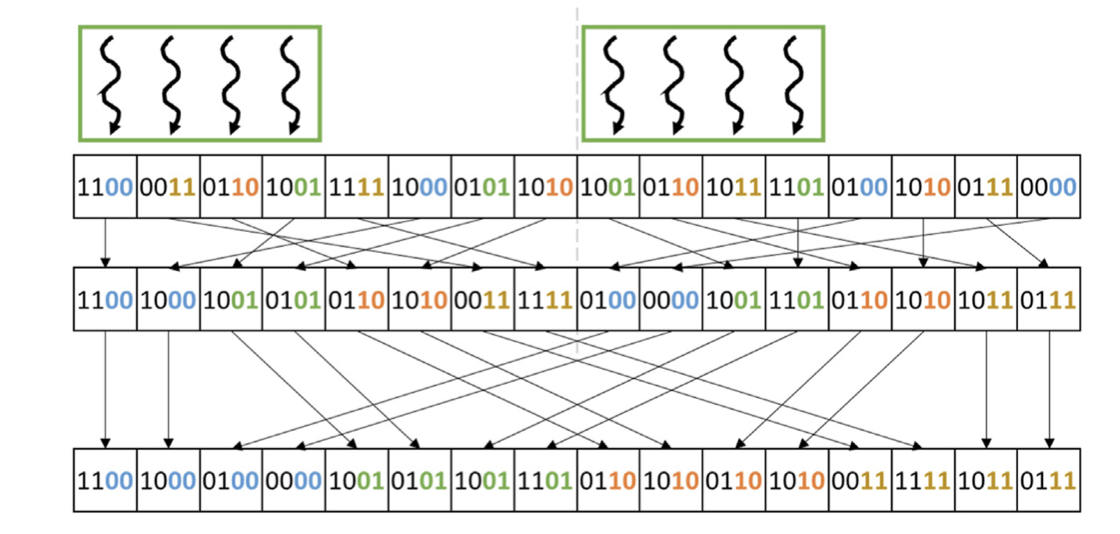
\includegraphics[width=0.9\textwidth]{figs/F13.10.png}
	\caption{\textit{常见 bug:在Buffer生存期内直接从主机分配中读取数据 }}
\end{figure}

为了避免这些错误,我们建议在开始使用带有 SYCL 的 C++ 时使用主机访问器而不是Buffer范围。 
主机访问器提供对主机Buffer的访问,一旦它们的构造函数完成运行,
我们就可以保证之前对Buffer的任何写入(例如,在创建 host\_accessor 之前提交的Kernel)都已执行并且可见。 
本书混合使用了两种风格(即主机访问器和传递给Buffer构造函数的主机分配)来熟悉这两种风格。 
开始时使用主机访问器往往不太容易出错。 图 13-11 显示了如何使用主机访问器从Kernel读取输出,而无需先破坏Buffer。

\begin{figure}[H]
	\centering
	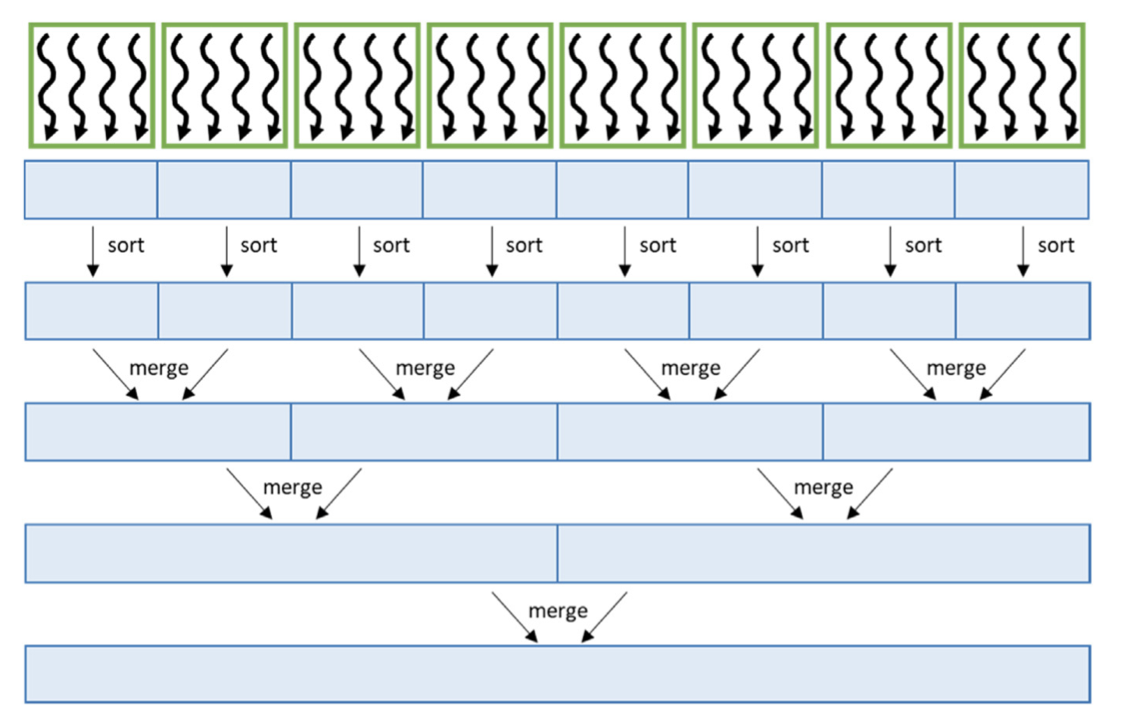
\includegraphics[width=0.9\textwidth]{figs/F13.11.png}
	\caption{\textit{建议:使用主机访问器读取Kernel结果 }}
\end{figure}

只要Buffer处于活动状态,例如在典型Buffer生命周期的两端,
就可以使用主机访问器 - 用于初始化Buffer内容并从Kernel读取结果。 图 13-12 显示了此模式的示例。

\begin{figure}[H]
	\centering
	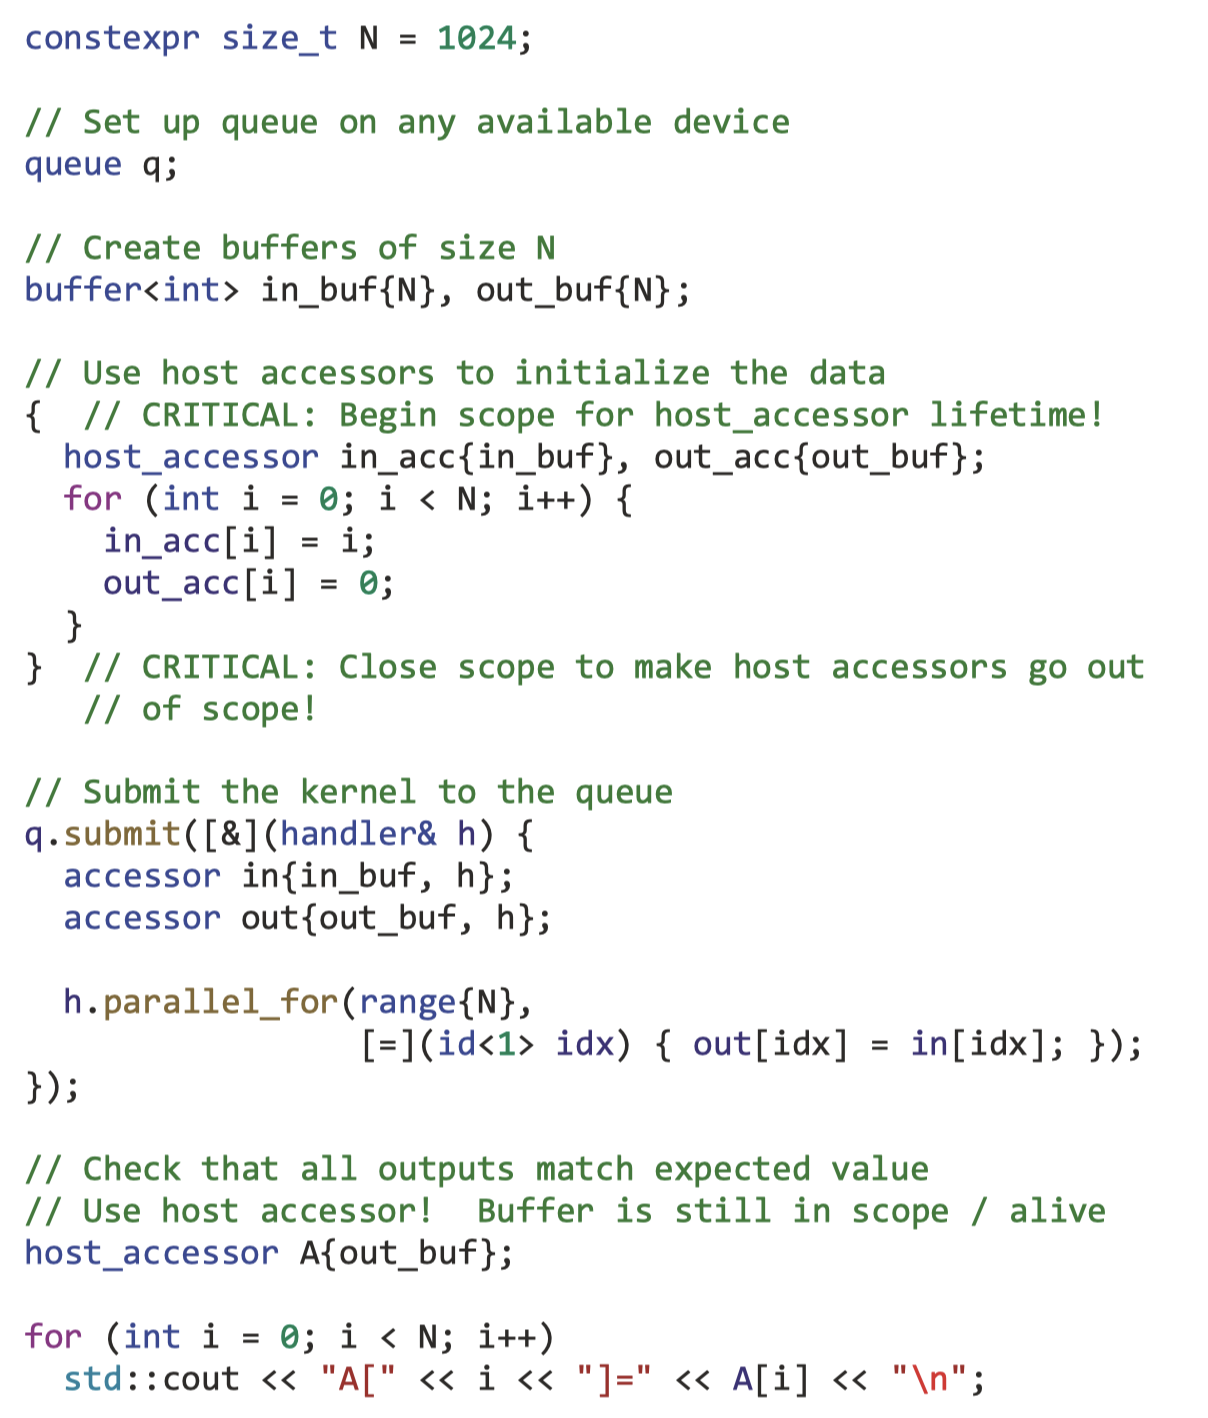
\includegraphics[width=0.9\textwidth]{figs/F13.12.png}
	\caption{\textit{建议:使用主机访问器进行Buffer初始化和结果读取 }}
\end{figure}

最后要提到的一个细节是,主机访问器有时会在应用程序中引起相反的错误,因为它们也有生命周期。 
当Buffer的主机访问器处于活动状态时,运行时将不允许任何设备使用该Buffer! 
运行时不会分析我们的主机程序来确定它们何时可以访问主机访问器,
因此它知道主机程序已完成访问Buffer的唯一方法是运行 host\_accessor 析构函数。 
如图 13-13 所示,如果我们的主机程序正在等待某些Kernel运行(例如,queue::wait() 或获取另一个主机访问器)
并且 SYCL 运行时正在等待某些Kernel运行,则这可能会导致应用程序挂起。 
我们早期的主机访问器在运行使用Buffer的Kernel之前会被销毁。

\begin{figure}[H]
	\centering
	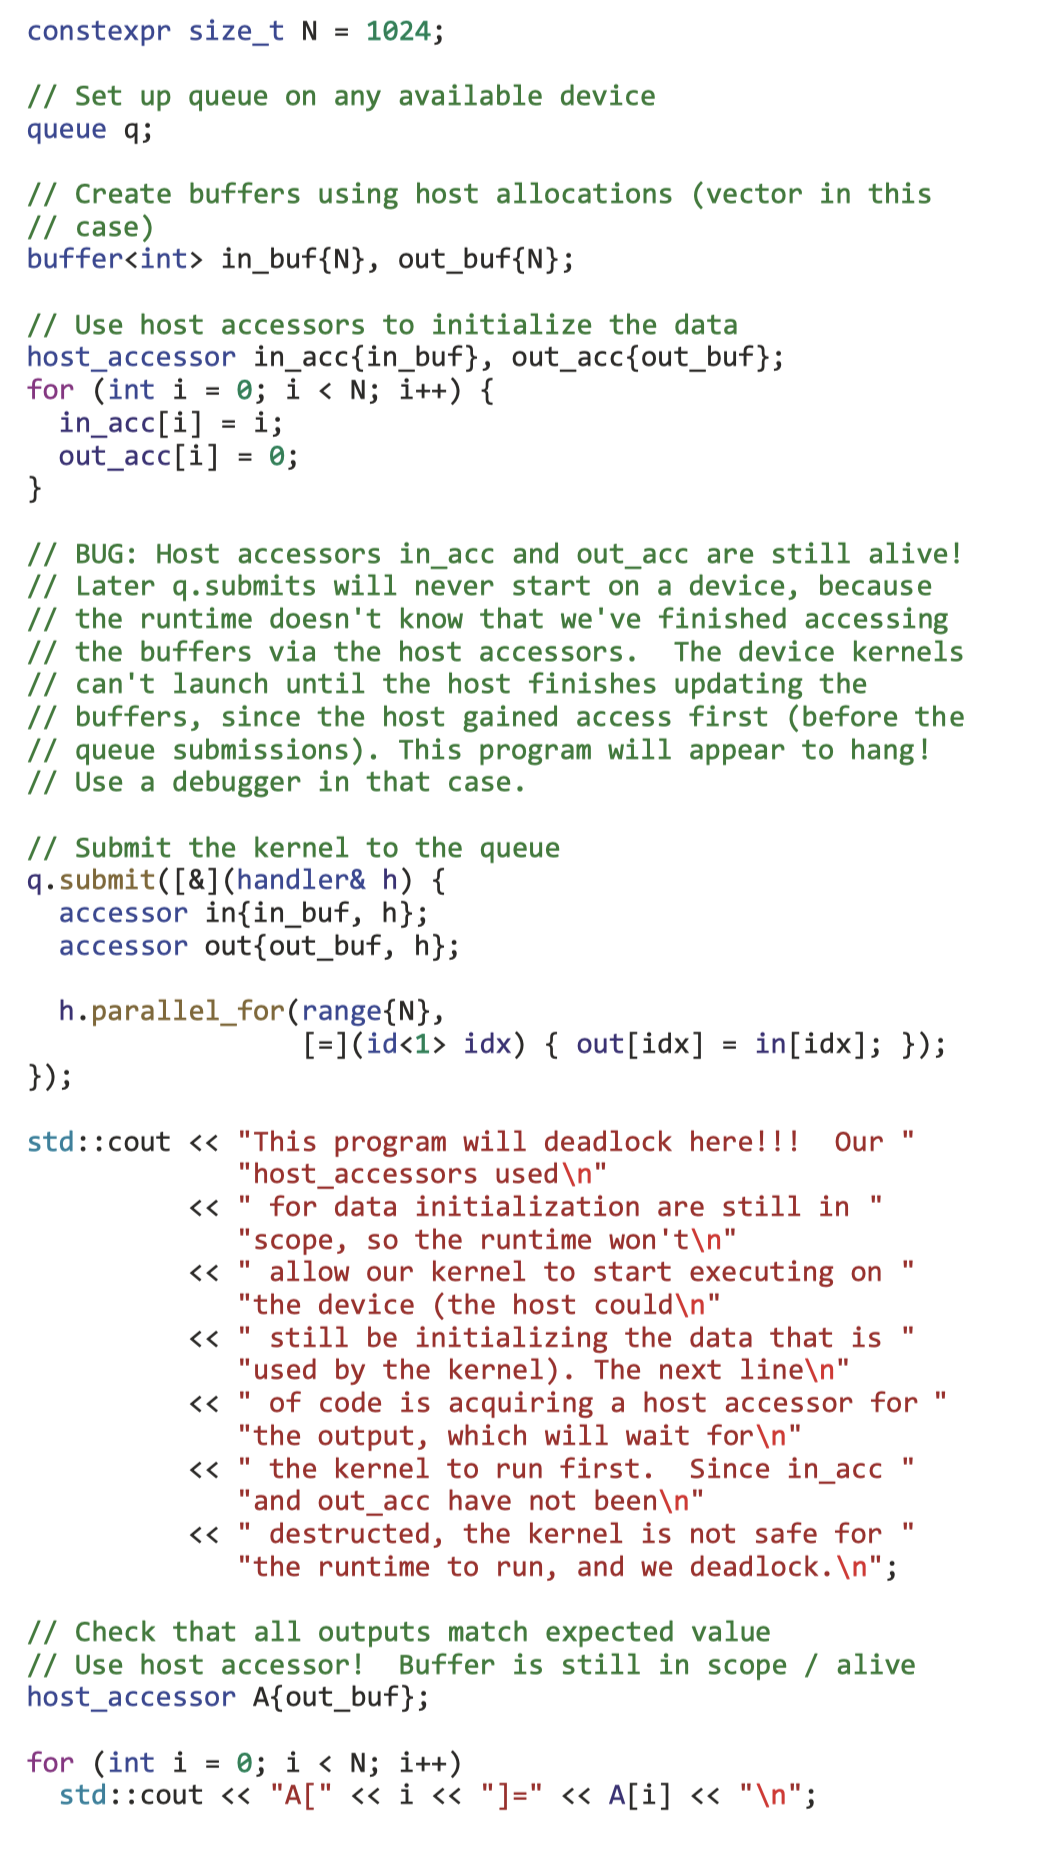
\includegraphics[width=0.9\textwidth]{figs/F13.13.png}
	\caption{\textit{由于不当使用 host\_accessor 而导致的死锁(错误 - 挂起!) }}
\end{figure}

\begin{remark}
	使用主机访问器时,请确保在不再需要Kernel或其他主机访问器解锁Buffer使用时销毁它们。
\end{remark}

\subsection{多个翻译单元}
当我们想要调用Kernel内部不同翻译单元中定义的函数时,这些函数需要使用 SYCL\_EXTERNAL 进行标记。 
如果没有这种修饰,编译器将仅编译在设备代码外部使用的函数(使得从设备代码内调用该外部函数是非法的)。

如果我们在同一翻译单元中定义函数,则 SYCL\_EXTERNAL 函数有一些限制不适用:

\begin{itemize}
	\item SYCL\_EXTERNAL 只能用于函数。

	\item SYCL\_EXTERNAL 函数不能使用原始指针作为参数或返回类型。 必须改用显式指针类。

	\item SYCL\_EXTERNAL 函数无法调用parallel\_for\_work\_item 方法。

	\item 不能从parallel\_for\_work\_group 范围内调用SYCL\_EXTERNAL 函数。
\end{itemize}

如果我们尝试编译一个调用不在同一翻译单元内且未使用 SYCL\_EXTERNAL 声明的函数的Kernel,
那么我们可以预期会出现类似于以下内容的编译错误:

error: SYCL kernel cannot call an undefined function without SYCL\_EXTERNAL attribute

如果函数本身是在没有 SYCL\_EXTERNAL 属性的情况下编译的,我们可以预期会看到链接或运行时失败,例如

terminate called after throwing an instance of '...compile\_program\_error'...

error: undefined reference to ...

SYCL不要求编译器支持SYCL\_EXTERNAL; 一般来说,它是一个可选功能。 DPC++ 支持 SYCL\_EXTERNAL。

\subsubsection{多个翻译单元的性能影响}
编译模型的含义(请参阅本章前面的内容)是,如果我们将设备代码分散到多个翻译单元中,
则与设备代码共置相比,可能会触发更多的即时编译调用。 
这高度依赖于实现,并且随着实现的成熟,可能会随着时间的推移而发生变化。

这种对性能的影响很小,足以在我们的大部分开发工作中忽略,但是当我们进行微调以最大限度地提高代码性能时,
我们可以考虑以下两件事来减轻这些影响:(1)将设备代码组合在一起 相同的翻译单元,
以及(2)使用提前编译来完全避免即时编译效应。 
由于这两者都需要我们付出一些努力,因此我们只有在完成开发并试图从应用程序中榨取每一盎司性能时才这样做。 
当我们确实采取这种详细的调整时,值得测试更改以观察它们对我们正在使用的确切 SYCL 实现的影响。

\subsection{当匿名 Lambda 需要名称时}
SYCL 允许为 lambda 分配名称,以防工具需要它并用于调试目的(例如,以用户定义的名称启用显示)。 
根据 SYCL 2020 规范,命名 lambda 是可选的。 
在本书的大部分内容中,匿名 lambda 都用于Kernel,
因为在使用 C++ 和 SYCL 时不需要名称(除了传递编译选项,如第 10 章中 lambda 命名讨论所述)。

当我们需要在代码库中混合来自多个供应商的 SYCL 工具时,该工具可能要求我们命名 lambda。 
这是通过将 <class uniquename> 添加到使用 lambda 的 SYCL 操作构造(例如,parallel\_for)来完成的。 
这种命名允许来自多个供应商的工具在单个编译中以定义的方式进行交互,
并且还可以通过显示我们在调试工具和层中定义的Kernel名称来提供帮助。

如果我们想使用Kernel查询,我们还需要命名Kernel。 
SYCL 标准委员会无法在 SYCL 2020 标准中找到解决方案来满足这一要求。 
例如,查询Kernel的preferred\_work\_group\_size\_multiple需要我们调用Kernel类的get\_info()成员函数,
这需要Kernel类的实例,这最终需要我们知道Kernel的名称(和kernel\_id)才能提取 来自相关 kernel\_bundle 的句柄。

\subsection{总结}
当今的流行文化经常将技巧称为生活窍门。 
不幸的是,编程文化常常给 hack 赋予负面含义,因此作者没有将本章命名为“SYCL Hacks”。 
毫无疑问,本章只是触及了使用 C++ 和 SYCL 的实用技巧的表面。 
当我们一起学习如何通过 SYCL 充分利用 C++ 时,我们所有人都可以分享更多技巧。